\section{Results} \label{RSS:sec:results}

We start by describing the tasks and our experimental methodology, then we present our results. These experiments are designed to show that training on augmentations generated by our method improves performance on a downstream task. We perform two simulated experiments, where we run thousands of evaluations, including several ablations (see Appendix 1.A). We also perform a real robot experiment (Figure \ref{RSS:fig:real_robot_setup}) where we run 30 iterations of online validity classifier learning, with augmentation and without. In all experiments, we train until convergence or for a fixed number of training steps. This ensures a fair comparison to training without augmentation, despite the differing number of unique training examples. In all experiments, we generate 25 augmentations per original example (See Appendix 1.B). We define key hyperparameters of our method in Appendix 1.C. A link to our code is available on the \href{https://sites.google.com/view/data-augmentation4manipulation}{project website}.

\subsection{Cluttered Planar Pushing}

\begin{figure}
    \centering
    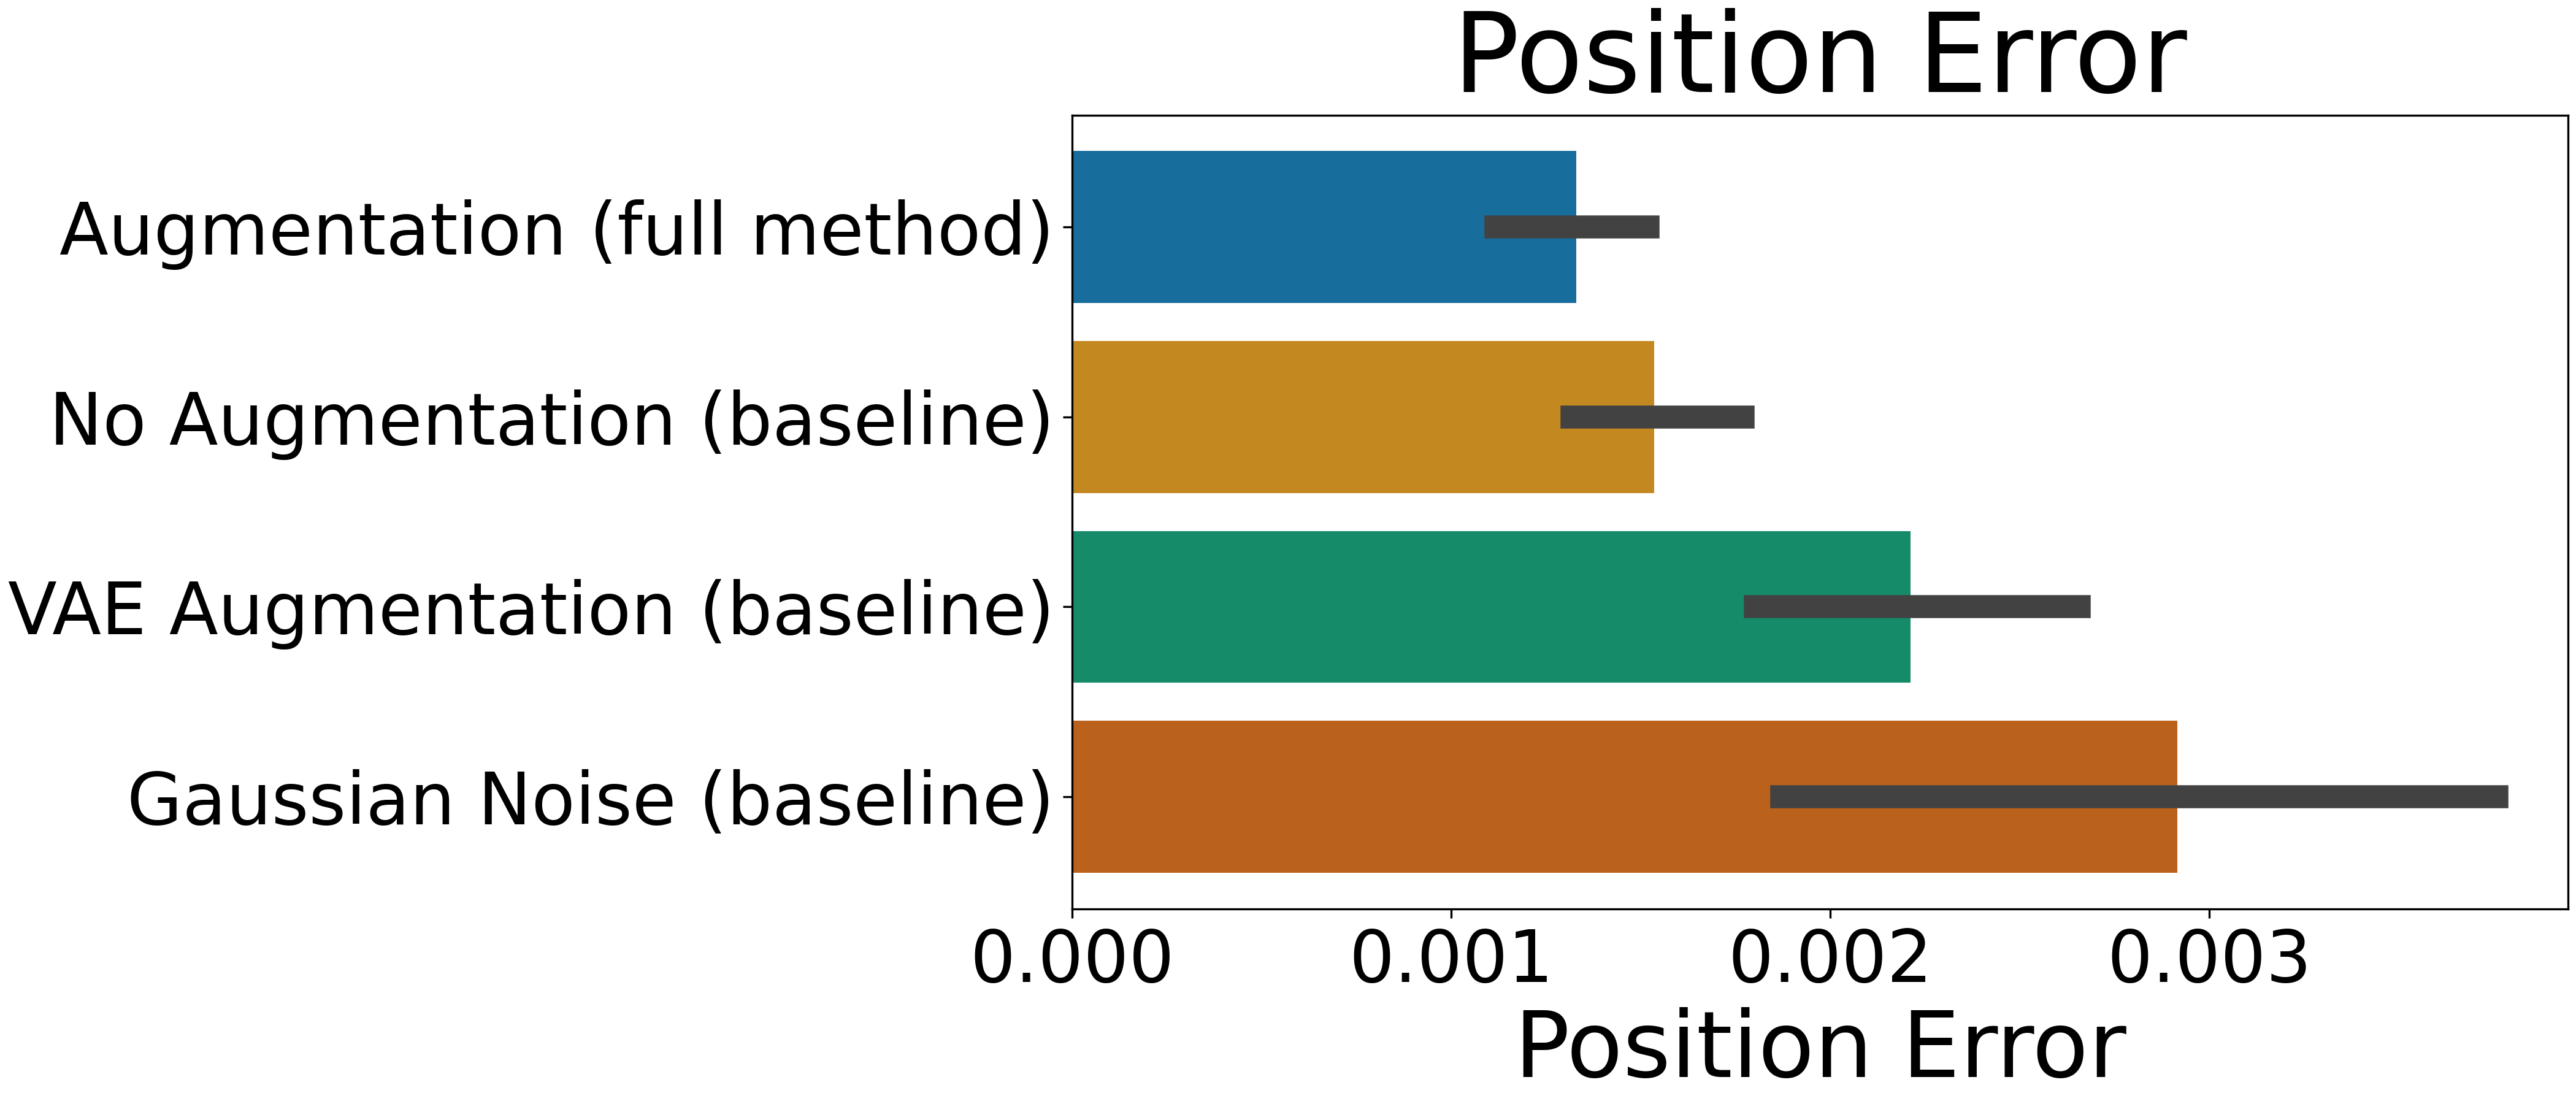
\includegraphics[width=0.7\linewidth]{Chap3/images/cylinders_results1.png}
    \caption{Mean position error (meters) for learning the dynamics of cluttered planar pushing.}
    \label{RSS:fig:cylinders_results}
\end{figure}

The cluttered planar pushing environment consists of a single robotic arm pushing 9 cylinders around on a table. The task is to learn the dynamics, so that the motion of the cylinders can be predicted given initial conditions and a sequence of robot actions. For this, we use PropNet \cite{Propnet}, and our task is inspired by the application of PropNet to planar pushing in \cite{DBRP2020}. The inputs to PropNet are an initial state $\state_0$ and a sequence of actions $\baction$, and the targets are the future state $(\state_1,\dots,\state_T$). All trajectories are of length 50. We evaluate the learned dynamics by computing the mean and maximum errors for position and velocity on a held-out test set. Example augmentations for this scenario are shown in Figure \ref{RSS:fig:cylinders_aug_examples}. 

This is an interesting application of our augmentation for several reasons. First, it is a regression task, which few augmentation methods allow. Second, the output of the dynamics network is high-dimensional (900 for a prediction of length 50), which normally means large datasets are needed and engineering invariances into the data or network is difficult. Finally, the trajectories contain non-negligible velocities and are not quasi-static.

\begin{figure}
    \centering
    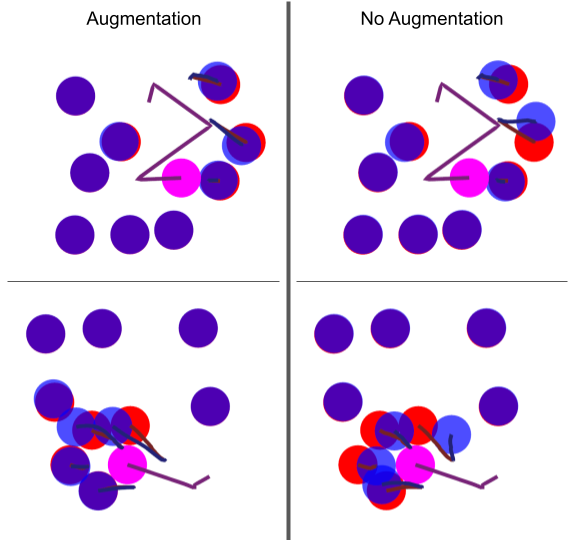
\includegraphics[width=0.6\linewidth]{Chap3/images/cylinders_rollouts.png}
    \caption{Predictions (blue) vs. ground truth (red) for planar pushing. The robot is in pink. Trajectories are visualized with lines. The left column shows predictions from a model trained with augmentation, the right column without.}
    \label{RSS:fig:cylinders_rollouts}
\end{figure}

The original dataset contained 60 trajectories of length 50, or \SI{3000} time steps in total. For comparison, previous work on the same dynamics learning problem used over \SI{100000} time steps in their datasets \cite{Propnet,DBRP2020}. This is similar to the number of training examples we have \textit{after} augmentation, which is \SI{75000} time steps. Finally, we measured the performance of our implementation and found that for the planar pushing scenario we generate 4.5 augmentations per second on average.

The primary results are shown in Figure \ref{RSS:fig:cylinders_results}. Augmentation reduces the average position error from \SI{0.00154}{\meter} to \SI{0.00133}{\meter}, a decrease of 14\%. Additionally, we include two baselines, one which adds Gaussian noise to the state, robot, action, and environment data, and one which uses a VAE to generate augmentations as in \cite{MaterialsAEOhno2020}. The magnitude of the Gaussian noise was chosen manually to be small but visually noticeable. Our proposed augmentation method is statistically significantly better than the baseline without augmentation ($p<0.0362$), the Gaussian noise baseline ($p<0.0001$), and the VAE baseline ($p<0.0002$). This difference in error may seem small, but note that error is averaged over objects, and most objects are stationary. Two roll-outs from with-augmentation and from without-augmentation are shown in Figure \ref{RSS:fig:cylinders_rollouts}. In particular, we found that augmentation reduces ``drift,'' where the model predicts small movements for objects that should be stationary. Finally, we note that the Gaussian noise and VAE baselines perform worse than no augmentation, suggesting that data augmentation can hurt performance if the augmentations are done poorly.

\subsection{Bimanual Rope Manipulation}

In this task, the end points of a rope are held by the robot in its grippers in a scene resembling the engine bay of a car, similar to \cite{UnreliableMitrano2021}, and shown in Figure \ref{RSS:fig:sim_envs}. The robot has two 7-dof arms attached to a 3-dof torso with parallel-jaw grippers. The tasks the robot performs in this scene mimic putting on or taking off lifting straps from the car engine, installing fluid hoses, or cable harnesses. These tasks require moving the strap/hose/cable through narrow passages and around protrusions to various specified goal positions without getting caught. One iteration consists of planning to the goal, executing open-loop, then repeating planning and execution until a timeout or the goal is reached. The goal is defined as a spherical region with \SI{4.5}{\centi\meter} radius, and is satisfied when any of the points on the rope are inside this region.

The planner is an RRT with a learned constraint checker for edge validity (validity classifier), and more details are given in \cite{UnreliableMitrano2021}. We want to learn a classifier that takes in a single transition $x = (\state_t,\action_t,\state_{t+1},\env_t)$ and predicts whether the transition is valid. Without a good constraint checker, the robot will plan trajectories that result in the rope being caught on obstacles or not reaching the goal. We apply our augmentation algorithm to the data for training this constraint checker. After an execution has completed, the newly-collected data along with all previously collected data are used to train the classifier until convergence. Example augmentations for this scenario are shown in Figure \ref{RSS:fig:rope_aug_examples}. The objective is to learn the constraint checker in as few iterations as possible, achieving a higher success rate with fewer data.

\begin{figure}
    \centering
    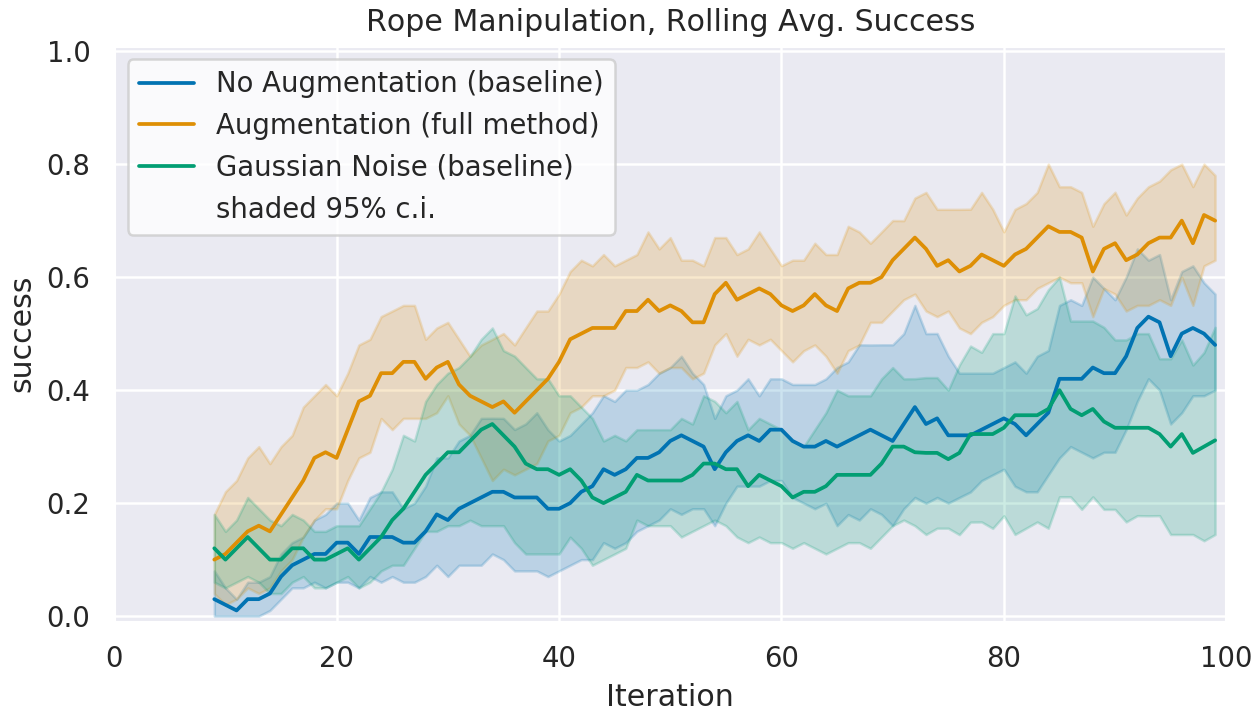
\includegraphics[width=1\linewidth]{Chap3/images/success_rate_rolling.png}
    \caption{The success rate on simulated bimanual rope manipulation, using a moving window average of 10.}
    \label{RSS:fig:rope_results}
\end{figure}

In this experiment, a total of \SI{3038} examples were gathered (before augmentation, averaged over the 10 repetitions). Since the purpose of our augmentations is to improve performance using small datasets, it is important that this number is small. In contrast, prior work learning a similar classifier used over \SI{100000} examples in their datasets \cite{UnreliableMitrano2021,UnreliableDale2019}. This is similar to the number of training examples we have \textit{after} augmentation, which is \SI{75950} on average.  Finally, we measured the performance of our implementation and found that for the rope scenario we generate 27 augmentations per second on average.

The primary results are shown in Figure \ref{RSS:fig:rope_results}. Over the course of 100 iterations, the success of our method using augmentation is higher than the baseline of not using augmentation, as well as the Gaussian noise baseline. We omit the VAE baseline, since it performed poorly in the planer pushing experiment. Furthermore, it is computationally prohibitive to retrain the VAE at each iteration, and fine-tuning the VAE online tends to get stuck in bad local minima. The shaded regions show the 95th percentile over 10 runs. If we analyze the success rates averaged over the final 10 iterations, we find that without augmentation the success rate is 48\%, but with augmentation the success rate is 70\%. The Gaussian noise baseline has a final success rate of 31\%. A one-sided T-test confirms statistical significance ($p<0.001$ for both).

\subsection{Real Robot Results}
\label{RSS:sec:real_robot_results}

\begin{figure}
    \centering
    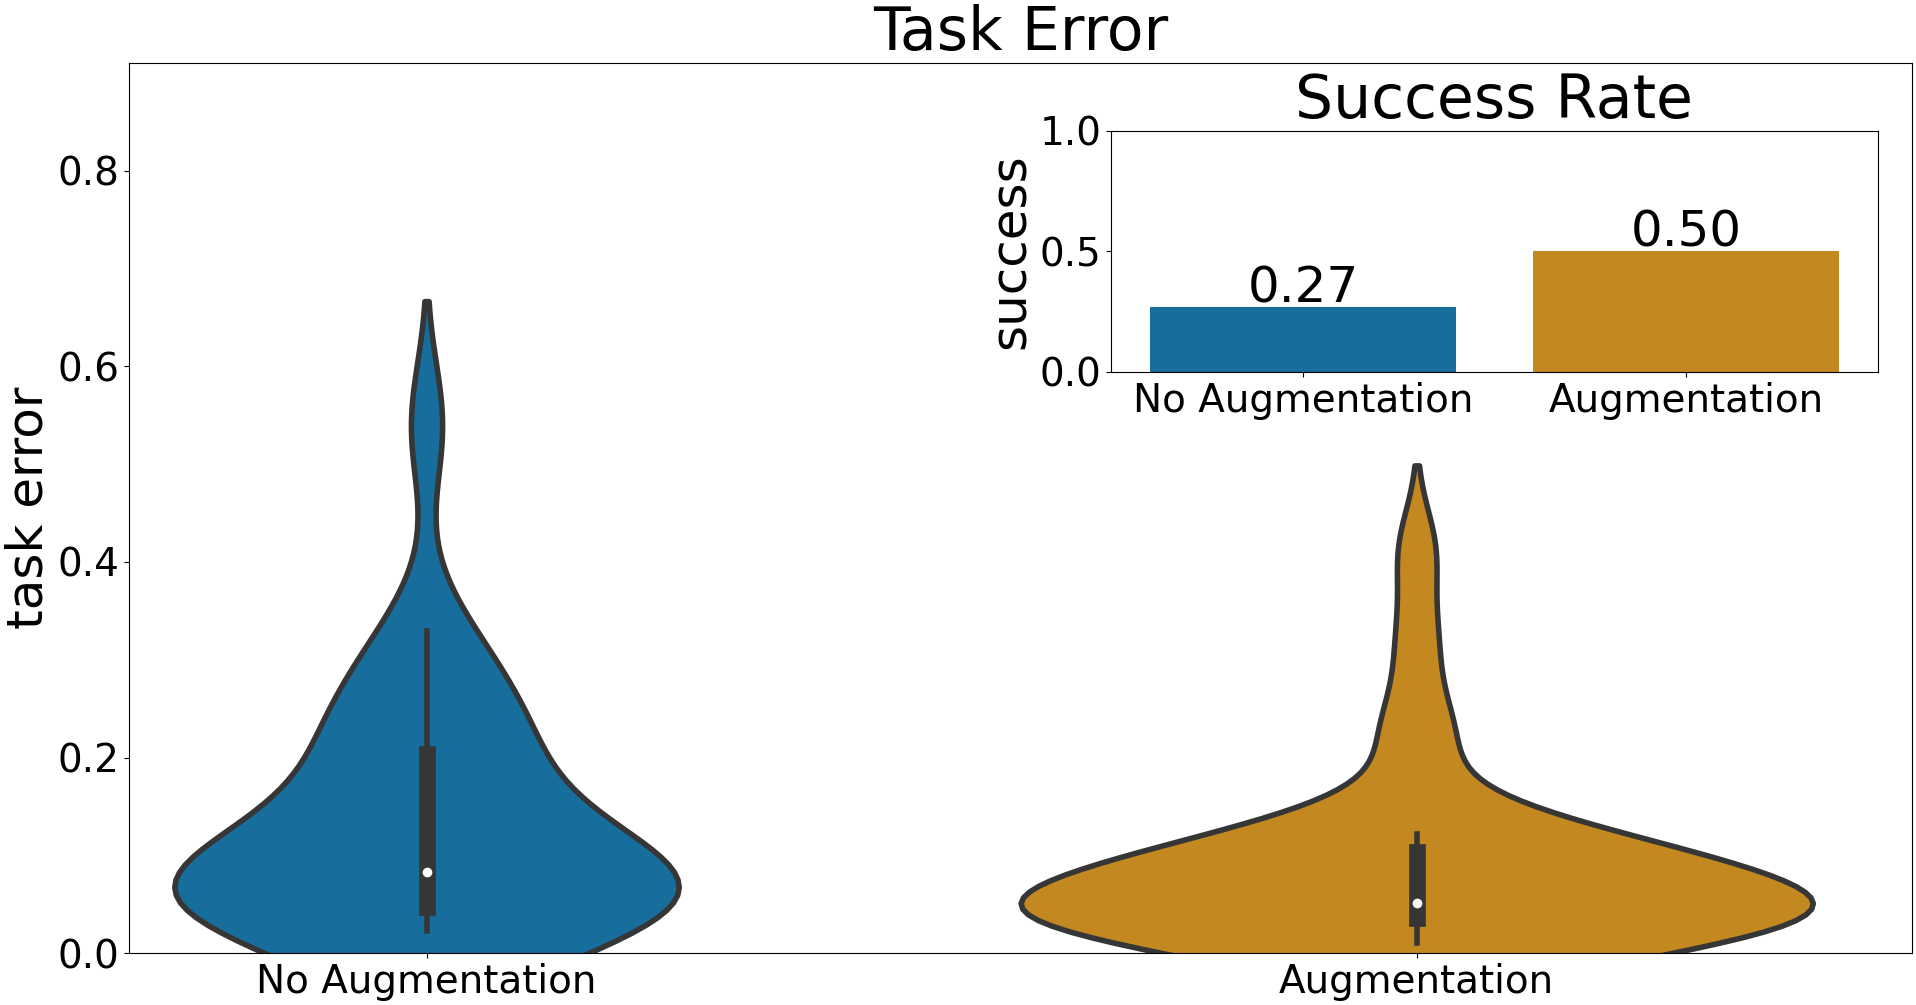
\includegraphics[width=0.7\linewidth]{Chap3/images/real_robot_task_error_success.png}
    \caption{The success rate and task error distribution of bimanual rope manipulation on the real robot. Task error is the distance between the goal and the final observed state of the rope.}
    \label{RSS:fig:real_robot_results}
\end{figure}

In this section, we perform a similar experiment to the simulated bimanual rope manipulation experiment, but on real robot hardware. This demonstrates that our method is also effective on noisy sensor data. More importantly, it demonstrates how augmentation enables a robot to quickly learn a task in the real world. We use CDCPD2 \cite{CDCPD2} to track the rope state. The geometry of the car scene is approximated with primitive geometric shapes, like in the simulated car environment.

We ran the validity classifier learning procedure with a single start configuration and a single goal region, both with and without augmentation. After 30 iterations of learning, we stop and evaluate the learned classifiers several times. With augmentation, the robot successfully placed the rope under the engine 13/26 times. Without augmentation, it succeeded 7/26 times. The Gaussian noise and VAE baselines performs poorly in simulated experiments, therefore we omit them in the real robot experiments.
